\section{Experiment}

This work presents the results of several experiments, dedicated to the $^{6,7}$H studies and one reference measurement of the same reaction mechanism, performed to control all the setup parameters and to test the reliability of the obtained results.
All the experiments were conducted in at the ACCULINNA-2 fragment separator \cite{Fomichev:2018}, recently constructed in the Flerov Laboratory of Nuclear Reaction of the Joint Institute for Nuclear Research. 
In this chapter, one briefly presents the main features of the ACCULINNA-2 facility and describes in more details the experimental setups, employed for the investigations of the isotopes of interest.

\subsection{ACCULINNA-2}

The idea of the ACCULINNA-2 in-flight separator is to provide low-energy (from 10 to 40\,AMeV) RIBs of high intensity and purity. 
One should not, that it is not appropriate to compare its properties with those of such large facilities as FRS \cite{geissel:1992} and SuperFRS \cite{geissel:2003,winkler:2008} at FAIR, ARIS at FRIB \cite{gao:2015}, BigRIPS at RIKEN \cite{kubo:2003}, or others \cite{cuttone:2007,www:ganil,www:isolde}.
The uniqueness of the ACCULINNA-2 facility is illustrated in Fig.\ \ref{fig:acculinna2_worldplace}.
One may see, that among all other in-flight separators, the chosen one is able to provide the light RIBs of the lowest possible energy, which is indispensable for certain experimental issues.
The technical approach of the facility allows one to provide a high energy and angular resolution of the secondary beams, which in conjunction with high efficiency for correlation measurements allows user to analyse multiple kinematic conditions of the projectile and the reaction products.  
That is why, selection of the studied reaction channel can be easily carried out, which, afterwards, leads to high quality spin-parity identification for the excitation spectra of the systems of interest.

%-------------------------------------------------------------------------------
\begin{figure}[t]
	\begin{center}
		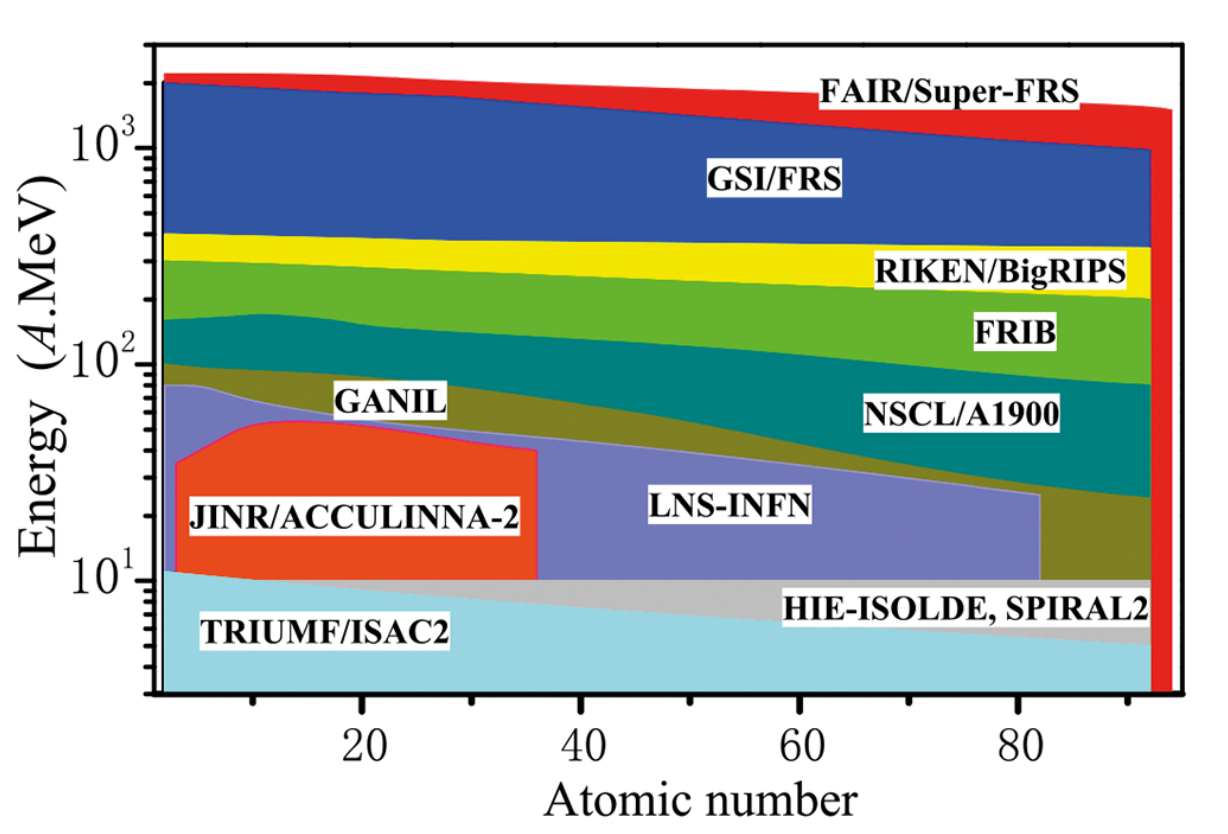
\includegraphics[width=0.7\textwidth]{figures/acculinna2_part.png}
	\end{center}
	%
	\caption{
		Landscape of the present-day facilities on the diagram where for radioactive beams, specified in terms of their atomic numbers, the available RIB energy ranges are shown.}
	%
	\label{fig:acculinna2_worldplace}
\end{figure}
%-------------------------------------------------------------------------------

The ACCULINNA-2 facility is coupled to the U400-M cyclotron and intended for production the RIBs by in-flight method, their separation and transport. 
It is also can be configured to form the stable beams, derived by the cyclotron.
The ACCULINNA-2 facility is 36 meters long achromatic separator consisting of two 45-degree dipole magnets, 14 quadrupoles, eight multipoles (three octupoles and five sextupoles) and four steering magnets, see Fig.\ \ref{fig:acculinna2_scheme}.
The high intensity primary beams are delivered by the U-400M cyclotron to the rotating production target module installed in the first intermediate focal plane F1 to produce radioactive ion beams in fragmentation reactions via the in-flight method.

The target module integrates a vacuum chamber with a water cooled beryllium target mounted on rotating magnetic liquid feed through and a set of water-cooled diaphragms. 
The target module is designed to work with heating power up to 2\,kW. 
Using the combination of magnetic analysis and energy losses in achromatic wedge degrader located at the intermediate dispersive focal plane F2, the secondary ions are separated in flight. 
Then, the secondary beam is delivered into the low-background experimental area with full particle-by-particle identification.

%-------------------------------------------------------------------------------
\begin{figure}[t]
	\begin{center}
		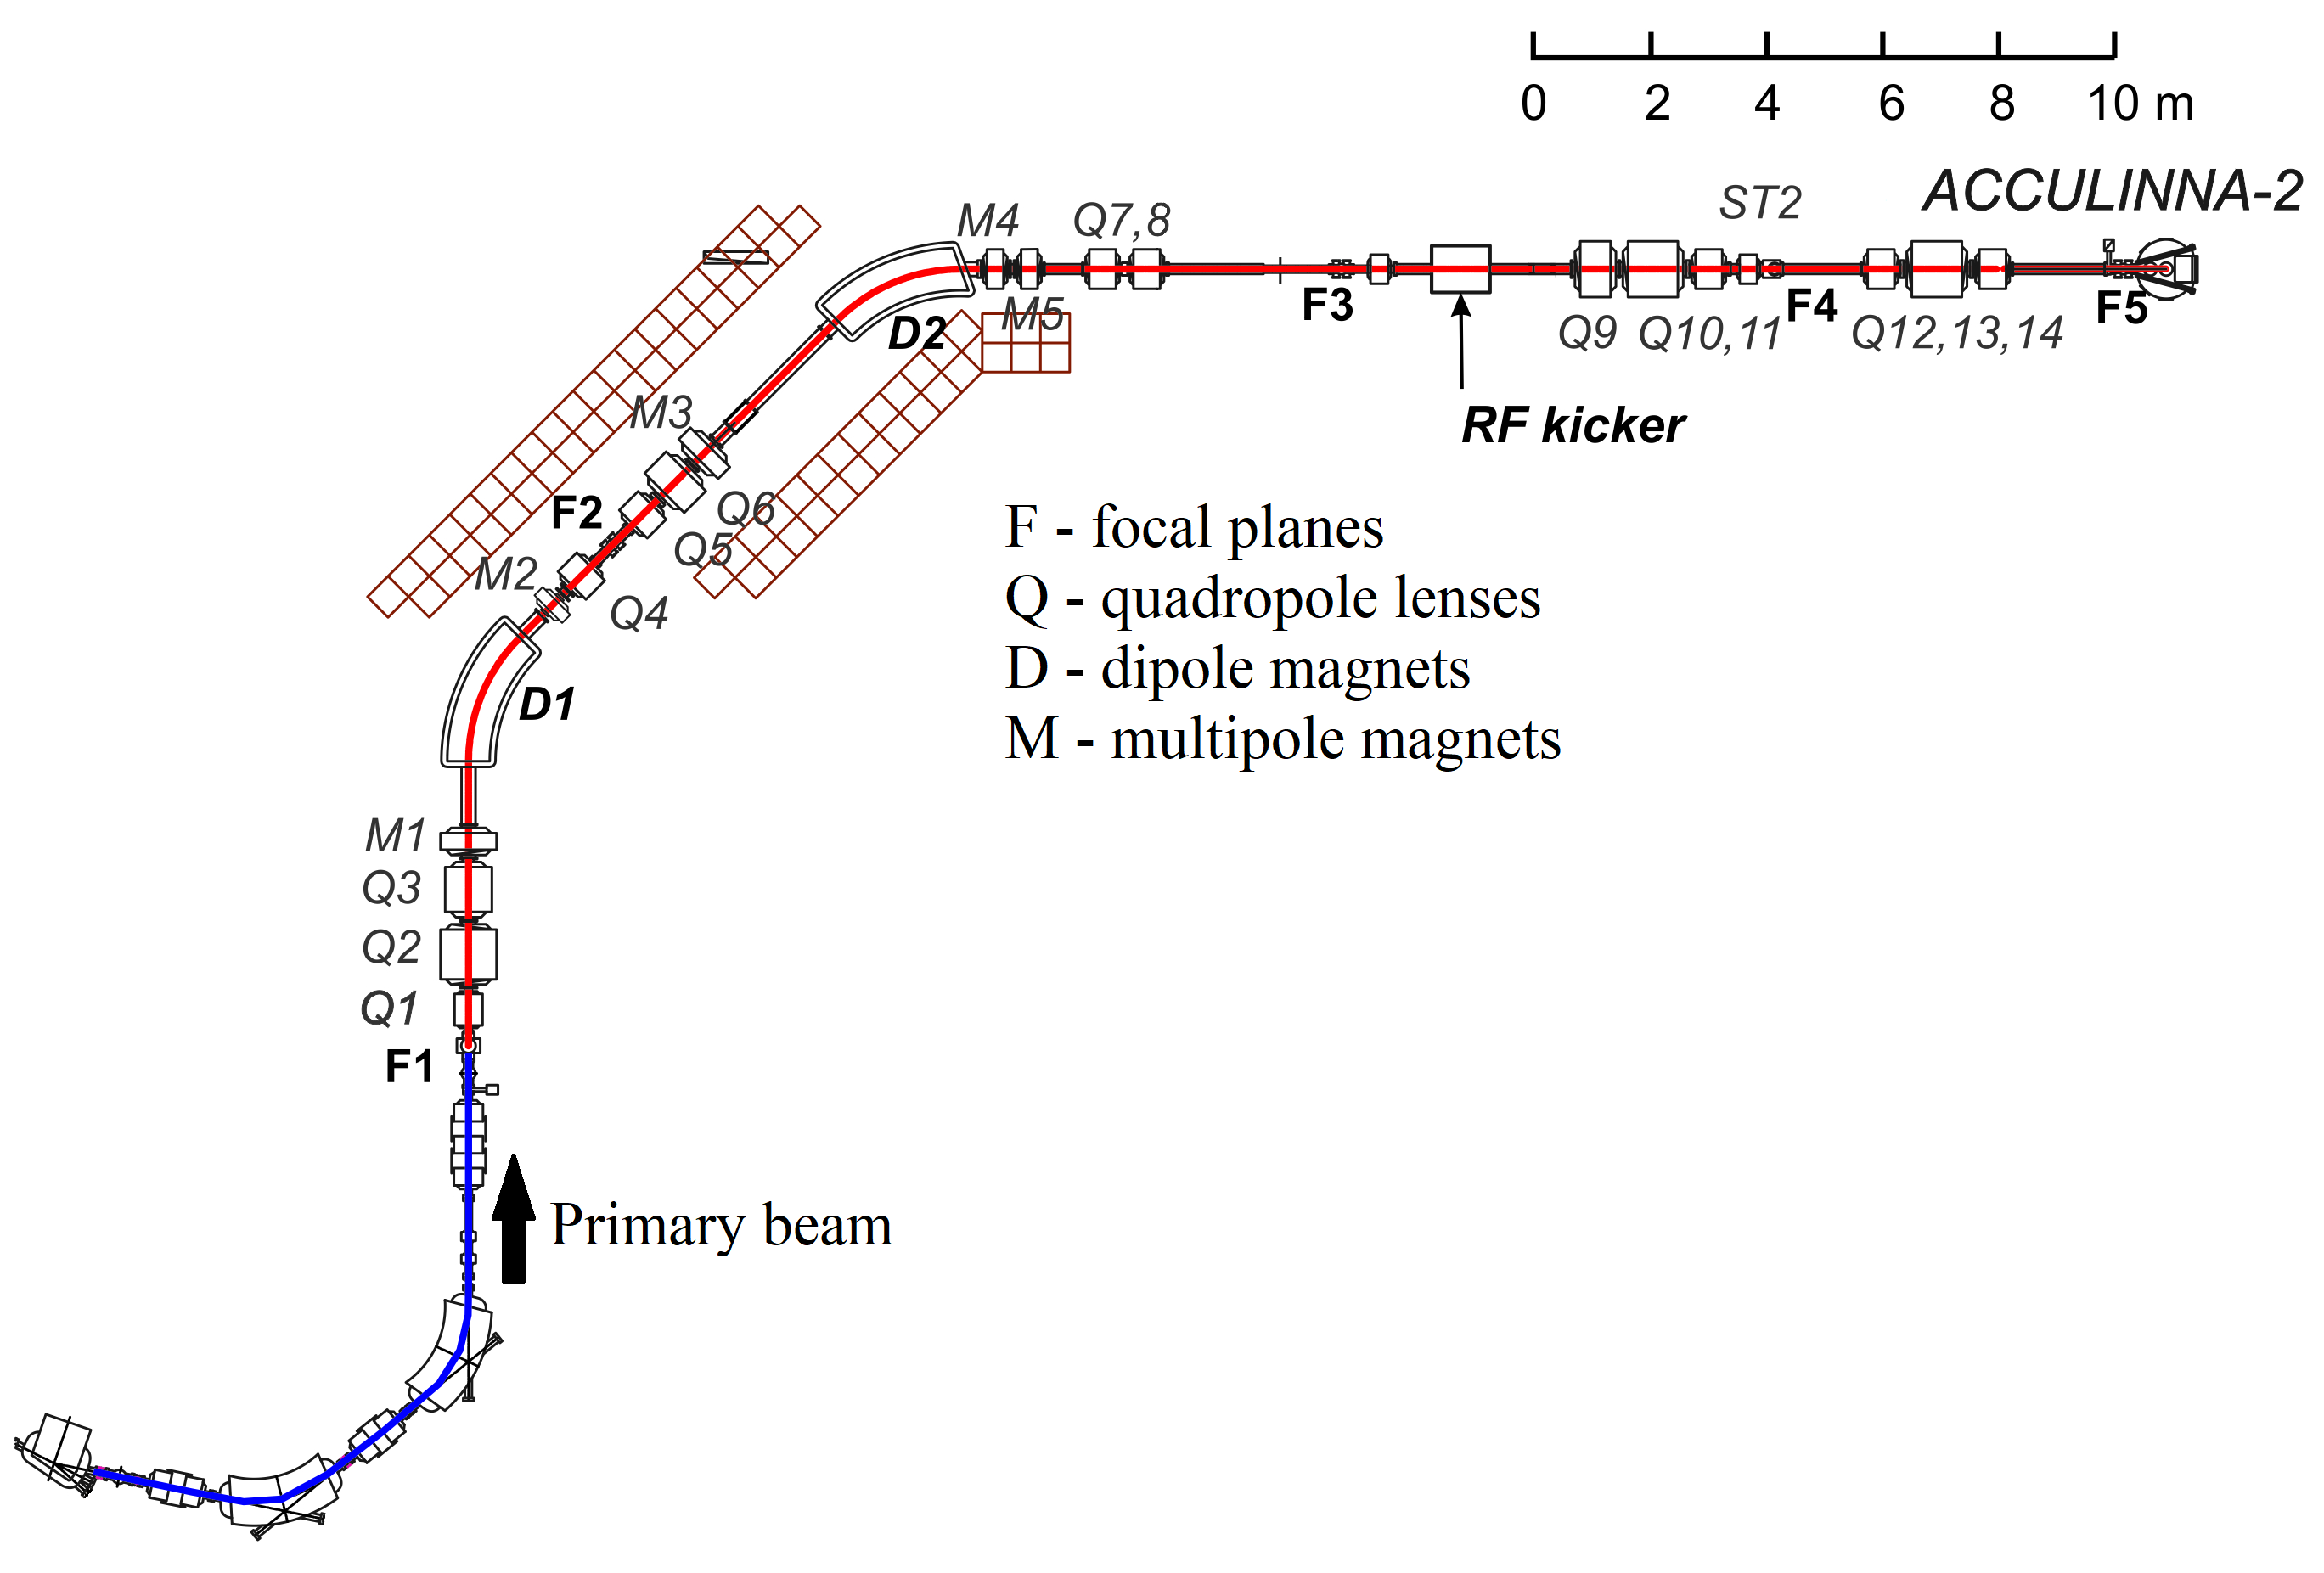
\includegraphics[width=1\textwidth]{figures/acculinna2.png}
	\end{center}
	%
	\caption{Lay-out of the fragment-separator ACCULINNA-2. F1 – the object plane; F2 – the intermediate dispersion plane; F3, F4 – the achromatic focal planes; F5 – the final focal plane.}
	%
	\label{fig:acculinna2_scheme}
\end{figure}
%-------------------------------------------------------------------------------



